\documentclass[conference]{IEEEtran}


\usepackage{cite}
\usepackage{pslatex} % -- times instead of computer modern, especially for the plain article class
\usepackage[colorlinks=false,bookmarks=false]{hyperref}
\usepackage{booktabs}
\usepackage{graphicx}
\usepackage{xcolor}
\usepackage{multirow}
\usepackage{comment}
\usepackage{listings}
%\usepackage{flushend} % even out the last page, but use only at the end when there is a bibliography
%\usepackage{minted}		% For inserting code
%\setminted[systemverilog]{
%	tabsize=3
%}
%\setminted[C]{
%	tabsize=3,
%	breaklines
%}
%\setminted[scala]{
%	tabsize=3,
%	breaklines
%}
\usepackage{xspace}		% For using \SV with trailing spaces
\usepackage{cleveref}	% Needed for correctly referencing listings
\usepackage{subfig}

\newcommand{\code}[1]{{\small{\texttt{#1}}}}
\newcommand{\SV}{SystemVerilog\xspace}


% fatter TT font
\renewcommand*\ttdefault{txtt}
% another TT, suggested by Alex
% \usepackage{inconsolata}
% \usepackage[T1]{fontenc} % needed as well?

%\newcommand{\todo}[1]{{\emph{TODO: #1}}}
\newcommand{\todo}[1]{{\color{olive} TODO: #1}}
\newcommand{\martin}[1]{{\color{blue} Martin: #1}}
\newcommand{\simon}[1]{{\color{green} Simon: #1}}
\newcommand{\abcdef}[1]{{\color{red} Author2: #1}}
\newcommand{\rewrite}[1]{{\color{red} rewrite: #1}}
\newcommand{\ducky}[1]{{\color{orange} Richard: #1}}
\newcommand{\kasper}[1]{{\color{purple} Kasper: #1}}
\newcommand{\hjd}[1]{{\color{pink} Hans: #1}}

% uncomment following for final submission
%\renewcommand{\todo}[1]{}
%\renewcommand{\martin}[1]{}
%\renewcommand{\simon}[1]{}
%\renewcommand{\kasper}[1]{}
%\renewcommand{\ducky}[1]{}



%%% ZF
\usepackage{listings}
\lstset{
	columns=fullflexible,
	%        basicstyle=\ttfamily\footnotesize,
	basicstyle=\ttfamily\small,      
	%columns=fullflexible, keepspaces=true,
	numbers=left,    
	numberblanklines=false,
	captionpos=b,
	%	breaklines=true,
	escapeinside={@}{@},
	numbersep=5pt,
	language=C,
	tabsize=2,
	breakatwhitespace=true,
	breaklines=true,
	deletekeywords={for},
	%        keywordstyle=\ttfamily
	numbersep=5pt,
	xleftmargin=.10in,
	%xrightmargin=.25in
}

\newcommand{\longlist}[3]{{\lstinputlisting[float, caption={#2}, label={#3}, frame=tb, captionpos=b]{#1}}}

\title{ChiselVerify: An Open-Source Hardware Verification Library for
Chisel and Scala}

%\author{
%\IEEEauthorblockN{No Author Given}
%\IEEEauthorblockA{No Institute Given}
%}

\author{\IEEEauthorblockN{Andrew Dobis\IEEEauthorrefmark{1}, Tjark Petersen\IEEEauthorrefmark{1}, Hans Jakob Damsgaard\IEEEauthorrefmark{1}, Kasper Juul Hesse Rasmussen\IEEEauthorrefmark{1}, \\
Enrico Tolotto\IEEEauthorrefmark{1}, Simon Thye Andersen\IEEEauthorrefmark{1}, Richard Lin\IEEEauthorrefmark{2}, Martin Schoeberl\IEEEauthorrefmark{1}}\\
\IEEEauthorblockA{\IEEEauthorrefmark{1}\textit{Department of Applied Mathematics and Computer Science} \\
\textit{Technical University of Denmark}\\
Lyngby, Denmark \\\\
\IEEEauthorrefmark{2}\textit{Department of Electrical Engineering and Computer Sciences} \\
\textit{UC Berkeley}\\
Berkeley, CA \\\\
adobis@student.ethz.ch, s186083@student.dtu.dk, hans.damsgaard@tuni.fi, s183735@student.dtu.dk, \\
s190057@student.dtu.dk, simon.thye@gmail.com, richard.lin@berkeley.edu, masca@dtu.dk}
}


\begin{document}

\maketitle
\thispagestyle{empty}
\pagestyle{empty}


\begin{abstract}
Modern digital hardware is becoming ever more complex. The development of %Performance increase with general-purpose processors has come to a halt.
different application-specific accelerators rather than traditional %We can no longer depend on Moore's Law to increase computing performance.
general purpose processors calls for advanced development methods %The only way to achieve higher performance or lower energy consumption
not only for design, but equally so for subsequent verification. %is by building domain-specific hardware accelerators.
Recently, this has made engineers propose an agile hardware development flow. %To efficiently design and verify those domain-specific accelerators, we need
However, one of the main obstacles when proposing such a method is the lack of %agile hardware development. One of the main obstacles when proposing such a modern method
efficient tools. %is the lack of modern tools to attack it. To verify a design in such a time-constrained development
%method, one needs to have efficient tools both for design and verification.

Chisel, a high-level hardware construction language, was introduced in order to combat this lack.
Since this already enables agile hardware design, we instead focus our attention on the verification flow. %circuits described in Chisel. It builds on top of the Chisel
Thus, this paper proposes ChiselVerify, an open-source library for verifying %hardware construction language and uses Scala to drive the verification process.
circuits described in Chisel. It builds on top of Chisel and uses Scala to drive %ChiselVerify increases the productivity of the verification engineer by allowing hardware testing to be done in a modern high-level programming environment.
the verification process. The solution is well integrated into the existing Chisel 
universe, making it an extension of currently existing testing libraries.


%We implement ChiselVerify in a way inspired by the functionalities found in SystemVerilog. This allows one to use
%functional coverage, constrained-random verification, bus functional models, transaction-level modelling and much more
%during the verification process of a design in a contemporary high-level programming ecosystem.
\end{abstract}

\begin{IEEEkeywords}
digital design, verification, Chisel, Scala
\end{IEEEkeywords}

%\section{TODO}
%
%\begin{itemize}
%\item REVIEW 1: Re-write abstract and introduction - remove anything not related to verification. Remove negative wording on Verilog and VHDL. Re-consider necessity of section III.A and Fig. 2. Need for a more advanced use case.
%\item REVIEW 2: Include ChiselTest and ChiselVerify in Fig. 1. Re-write sections 4, 5 and 6, and ensure close connection to introduction. Add a few words on ChiselVerify as an agile development tool. Need for a more advanced use case (with comparison to UVM). Remove filler sentences.
%\item REVIEW 3: Prove claimed productivity increase.
%\item REVIEW 4: Need for a more advanced use case.
%\item REVIEW 5: Prove claimed productivity increase. Add table of available methods (section III).
%\end{itemize}

\section{Introduction}
\label{sec:introduction}

Over the past several years, hardware design has grown to be ever more complex.
The increased demand for high-performance computing systems has lead to a larger need for domain-specific hardware accelerators~\cite{domain-hw-acc:2020}.
The design of these accelerators is often complex, and their development is time-consuming and error-prone.
In order to combat this added time-constraint, we can learn from software development trends such as agile software development~\cite{agile:manifesto}, and adapt to agile hardware development~\cite{henn-patt:turing:2019}.
Chisel~\cite{chisel:dac2012}, a Scala-embedded hardware construction language, was introduced in order to move digital circuit description to a more software-like high-level language. 

Many hardware engineers are switching away from the traditional hardware description %A few years ago, the two main design languages, Verilog and VHDL, dominated the
languages (HDLs), i.e., VHDL and Verilog, to SystemVerilog. And while SystemVerilog %design and testing of digital circuits.
does extend Verilog with object-oriented features for verification, its hardware %%However, both languages are decades behind
description flow remains the same as with Verilog. Thus, it does not fit an agile %%modern languages for software development.
development flow. %However, compared to software development and testing, digital design and testing methods/tools 
Chisel attempts to solve these issues by providing full support for %We thus developed a method and concrete tools for agile hardware development.
functional and object-oriented programming. However, Chisel is missing efficient verification tools %ChiselVerify combines tools, languages, development, and testing methods from the last decades in
with limited functionality available in the corresponding ChiselTest package~\cite{chisel:tester2}. %software development and applies them to hardware design.

As such, we choose to base our work on Chisel and ChiselTest, and aim to raise %We developed a verification framework in Scala.
the tooling level for a digital design. We have developed a verification framework %This framework is inspired by the Universal Verification Method (UVM) but leverages Scala's conciseness with the
inspired by the Universal Verification Method (UVM), but implemented by leveraging %combination of object-oriented and functional programming.
Scala's conciseness and support for both object-oriented and functional programming. %An initial experiment of testing the accumulator circuit of the Leros processor~\cite{leros:arcs2019}
Our framework, ChiselVerify, supports both coverage-oriented and constrained %showed that a test written with UVM was about 800 lines of code, where a Scala-based
random verification (CRV) flows with more features than those available in UVM. %test was around 80 lines of code~\cite{verify:chisel:2020}.
%However, UVM supports more functionalities than a plain ChiselTest~\cite{chisel:tester2} in Scala.

As a showcase, we have verified an industrial use case, a min-heap, utilizing 
ChiselVerify to check as many features of the min-heap with as few lines of 
verification code as possible.

The main contribution of this paper is ChiselVerify~\footnote{https://github.com/chiselverify/chiselverify}, an open-source verification library for hardware designs.

The paper is organized into 6 sections.
Section II describes related work.
Section III describes background on hardware verification.
Section IV describes our solution for enabling verification in Chisel, namely ChiselVerify.
Section V explores ChiselVerify on an industry-provided use case.
Section VI concludes.

\section{Related Work}
%\todo{\url{https://capra.cs.cornell.edu/latte21/}}

SystemVerilog is an extension of Verilog. Many non-synthesizable extensions are intended
to write more advanced test-benches. SystemVerilog adds object-oriented programming
for those test-benches. However, in contrast to Chisel, the object-oriented addition cannot be
used for hardware description.
SystemVerilog offers certain constructs capable of gathering coverage information~\cite{spear2008systemverilog}, such as statement and functional coverage. 
When it comes to functional coverage, our solution differs in several ways from SystemVerilog. 
On top of range-based bins, ChiselVerify's \texttt{cover} constructs can take temporal relations into account, as well as generalized conditional bins that work using purely user-defined hit predicates.
This differs from SystemVerilog, which mainly focuses on bins that cover value ranges or transitions. 

The \textit{Universal Verification Methodology} (UVM) was created as a standardized way of writing test-benches on top of SystemVerilog. 
It allows for the creation of reusable test-benches (i.e., using the same test for multiple designs)~\cite{uvm2015}. 
However, it is inherently verbose, since even a simple test requires around 800 lines of SystemVerilog code. 
UVM thus requires a significant initial time-investment, but is reusable once it gets up and running. 
UVM's structure differs from most traditional test-benches, making it less accessible for newcomers than the simpler approach done by ChiselTest.

Other projects have also focused on applying software testing techniques to hardware verification. 
RFuzz~\cite{rfuzz2018} focuses on creating a generalized method that enables efficient ``coverage-guided fuzz mutational testing''. 
This method relies on FPGA-accelerated simulation and new solutions allowing for quick and deterministic memory resetting, to efficiently use fuzzing (i.e., randomized testing, where the random seeds are mutated depending on certain coverage results) on digital circuits. 
The coverage metrics used in this solution are automated and based on branch coverage. 
This work offers a different type of solution. 
While we work mostly on verification functionalities inside a language, RFuzz delivers an efficient way to use said functionalities in order to ameliorate testing. 
RFuzz uses functional coverage tools in order to guide its randomized testing. 
Current work is also being done, in the scope of the ChiselVerify project, on coverage driven mutational fuzzing for digital circuits, however this is out of the scope of this paper.

\texttt{Chisel3.formal}  is a formal verification package containing a set of tools and helpers for formally verifying Chisel modules~\cite{chisel:formal}. 
In contrast to ChiselVerify, \texttt{chisel3.formal} proposes way of testing based around defining a set of formal checks that a design must pass in order to be considered as correct. 
These checks can, for example, look like: \texttt{past(io.out, 1) (pastIoOut => \{ assert(io.out >= pastIoOut) \})} which guarantees that the current module will never decrease its output from one cycle to the next. 
These formal checks can then be verified by calling the \texttt{verify(module)} function. 

This approach is similar to software contracts in Scala, like the ones enabled by ScalaCheck~\cite{scalacheck}. 
The main difference between our solution and this one is that here the rules are written on a per-module basis and are thus directly linked to the Chisel code, while our solution focuses on checking that a suite of test-benches is testing the right things. 
The \texttt{chisel3.formal} package has also been extended in \texttt{kiwi-formal}~\cite{chisel:kiwi-formal} and \texttt{dank-formal}~\cite{chisel:dank-formal}, each adding their own additional formal rule templates. 

As far as we know, ChiselVerify is the only verification framework allowing for the easy use of verification functionalities, well integrated into the ChiselTest-Chisel ecosystem.

\section{Background}
\label{sec:background}

This section presents a brief overview of what hardware verification is. 
We also briefly present Chisel and the current solutions that exist in it with regards to the verification of digital designs.

\subsection{Verification of Digital Designs}
Verification of digital designs refers to the testing of a design before it has been taped-out~\cite{spear2008systemverilog}. 
SystemVerilog~\cite{SystemVerilog} is one of the main languages used for verification.
The language enables verification engineers to define constraint-driven randomized test-benches and define metrics to gather functional coverage data related to a test suite. 
However, being embedded in a low-level language makes writing tests quite complex. 
The three main verification features that we are interested in are: functional coverage, constrained random verification, and bus functional modeling.

\subsubsection{Functional Coverage}
One of the main tools used in verification is test coverage. 
This allows verification engineers to measure their progress throughout the testing process and understand how effective their tests are. 
In contrast to the more common statement coverage, which defines a quantitative measure of the testing progress \textit{``How many lines of code have been tested?''}, functional coverage gives a qualitative measure, \textit{``Which functionalities have we tested?''}~\cite{spear2008systemverilog}.
Functional coverage enables the measurement of how correctly the specification has been implemented. 
This is measured relative to a verification plan, which includes the following components:

\begin{itemize}
  \item \texttt{Bin}s: Ranges of values that should be tested for (i.e., expected values of a given port).
  \item \texttt{Cover} constructs: Ports that need to be sampled in the coverage report, defined using a set of \texttt{bin}s.
\end{itemize}

\begin{figure*}
  \centering
    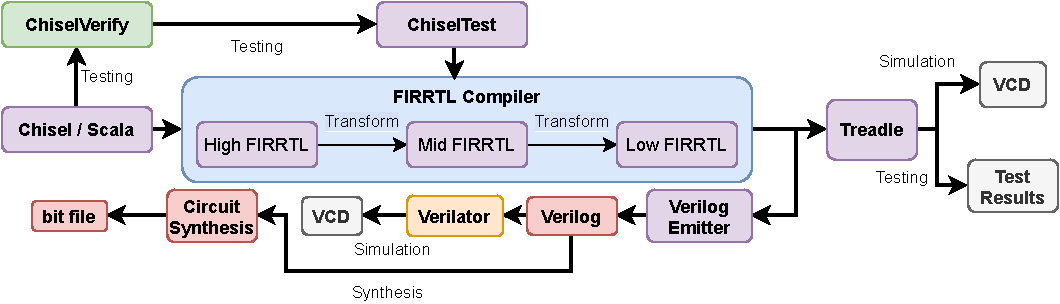
\includegraphics[width=0.8\linewidth]{Chisel_FIRRTL_VERILOG.pdf}
    \caption{Overview of the Chisel compilation pipeline.}
\label{fig:chisel-pipe}
\end{figure*}

\subsubsection{Constrained Random Verification}
CRV allows the verification engineer to create random variables which generate values that satisfy a set of associated constraints.
With constrained random inputs, a relatively small test suite can, statistically, cover many of a component's functionalities. 
In addition, the constraints help to ensure that no invalid input combinations that would not appear during regular operation are applied~\cite{MehtaCRV2018}.

These constraints define a constraint satisfaction problem (CSP).
CSP represents the entities of a problem as a finite homogeneous collection of constraints. 
CSP solvers thus serve as the basis for generating sets of constrained random signal values for verification.

SystemVerilog has native support for constrained random data types and a built-in CSP solver. 
Variables declared with the \texttt{rand} keyword are randomizable upon calling a \texttt{randomize} method.

\subsubsection{Bus Functional Models}
A bus functional model (BFM) is an abstract model of a (standardized) interface that enables interacting with manager or subordinate components at a transaction level rather than at the level of individual wires.
Many synthesis tools, including Xilinx's Vivado, provide IP generators whose output IP blocks are equipped with such interfaces. 
%Verification of components with such interfaces is most easily handled with these bus functional models (BFMs), which abstract reading and writing of signals to a transaction level. 
BFMs thus enable simpler, safer, and less verbose interactions with interfaces like, e.g., AXI.

\subsection{Digital Design with Chisel}
Our verification library is used for designs described in Chisel.
Chisel is a ``hardware construction language'' embedded in Scala, used to describe digital circuits~\cite{chisel:dac2012}.
This language is more high-level than the traditional hardware description languages, such as VHDL or Verilog, and enables object-oriented and functional programming in the context of digital design.

Since Chisel and Scala are executing on the Java virtual machine (JVM), they have an excellent interoperability with Java. 
We can therefore leverage a large pool of both Java and Scala libraries for hardware design and verification. 
Furthermore, the packaging system in Scala/Java simplifies the integration of external components.

Working in the JVM also allows for the use of the Java native interface, which enables JVM based languages to call C functions.
This enables co-simulations between Scala testers, Chisel designs, and a C-based golden model. 
This should allow companies to keep their existing C models, but move their simulation workflow into Scala/Chisel testers.

Chisel translates the hardware description into an intermediate representation called FIRRTL~\cite{firrtl}. 
It then performs multiple optimization stages, called transforms, during which high-level concepts, such as a functional map or vectors, are compiled into lower-level concepts that map onto what we usually see in a Verilog or VHDL description. 
Once that is done, the newly transformed FIRRTL, called Low FIRRTL, can be used either for simulation, using an execution engine such as Treadle, or for synthesis by translating it into Verilog, which is then used to generate the synthesized circuit. 
Note that the final Verilog description may also be used for simulation purposes using engines such as Verilator~\cite{verilator}. 
Figure~\ref{fig:chisel-pipe} shows an overview of the Chisel compilation pipeline.

\subsection{Testing Chisel Designs}
A digital design described in Chisel can be tested with ChiselTest~\cite{chisel:tester2}, a non-synthesizable testing framework for Chisel.
ChiselTest emphasizes on usability and simplicity while providing ways to scale up in complexity.
Fundamentally, ChiselTest is a Scala library that provides access into the simulator through
operations like \texttt{poke} (write value into circuit), \texttt{peek} (read value from circuit), and \texttt{step} (advance time).
As such, tests written in ChiselTest are just Scala programs, imperative code that runs one line after the next.

ChiselTest is missing fundamental verification functionalities that can improve the verification efficiency of Chisel designs. 
It is currently not possible to do things such as constrained random testing or obtaining functional coverage results while solely relying on the ChiselTest framework. 
Functionalities such as those are crucial when it comes to efficiently verify one's design.

\section{Verification with Chisel}

We propose ChiselVerify, a verification library written in Scala. 
ChiselVerify uses the device under test (DUT) interfacing features from ChiselTest in order to enable three main verification functionalities in Chisel: functional coverage, constrained random verification, and bus functional modelling. 
We also show how our framework can be used to create a bus functional model by creating one for the standardized AXI4 interface. 
The following subsections explain each functionality and present how to use it.

\subsection{Coverage in Chisel}
Our solution enables one to define functional coverage constructs for Chisel designs in Scala.
In order to implement the different components needed for functional coverage in Scala, we needed to be able to do the following:

\begin{itemize}
  \item Define a verification plan, using \texttt{cover} constructs.
  \item Sample DUT ports, using the ChiselTest framework.
  \item Keep track of bins to sampled value matches, using a coverage database.
  \item Compile all of the results into a comprehensible coverage report.
\end{itemize}

Implementing these elements was done using a structure based around a top-level element known as the \texttt{CoverageReporter}, enabling one to define a verification plan using a \texttt{register} method. 
This method stores \texttt{cover} construct to \texttt{bin} mappings inside a \texttt{CoverageDB} (DB being short for a database) object. 
Once the verification plan is defined, ports are sampled using the \texttt{sample} method, which is implemented using ChiselTest's peeking capabilities. 
Finally, at the end of a test suite, a functional coverage report is generated using the \texttt{report} method, which compiles the results stored in the database into a Scala \texttt{case class} which can be used to obtain coverage percentages and bin hit counts.

\begin{lstlisting}[captionpos=b,caption={Small Verification Plan defined using 3 \texttt{cover} constructs, including one cross coverage construct},label={lst:basicfuncov},language=scala]
val cr = new CoverageReporter
cr.register(
  cover("accu", dut.io.accu)(
    bin("lo10", 0 to 9),
    bin("First100", 0 to 99)),
  cover("test", dut.io.test)(
    bin("testLo10", 0 to 9)),
  cover("accuAndTest", dut.io.accu, dut.io.test)(
    cross("both1", 1 to 1, 1 to 1))
\end{lstlisting}

Listing~\ref{lst:basicfuncov} is an example of how to define a verification plan using our functional coverage tool. 
One concept used here is \textit{cross coverage}m defined using a \texttt{cover} construct on multiple ports. 
Cross coverage allows one to specify coverage relations between different ports. 
This means that a cross defined between, e.g., \texttt{dut.io.a} and \texttt{dut.io.b} will be used to gather information about when \texttt{a} and \texttt{b} cover specific values simultaneously~\cite{spear2008systemverilog}.
In listing~\ref{lst:basicfuncov}, we are checking that \texttt{accu} and \texttt{test} take the value 1 at the same time.

Once our verification plan is defined, we need to decide when we want to sample our cover points using our coverage reporter.
This can be done, in our example, simply by calling \texttt{cr.sample()} when we are ready to sample our points. 
Finally once our tests are done, we can ask for a printed coverage report by calling \texttt{cr.printReport()} which results in the following: 
\begin{verbatim}
=============== COVERAGE REPORT ===============
================= GROUP ID: 1 =================
COVER_POINT PORT NAME: accu
BIN lo10 COVERING 0 to 9 HAS 8 HIT(S) = 80%
BIN First100 COVERING 0 to 99 HAS 9 HIT(S) = 9%
===============================================
COVER_POINT PORT NAME: test
BIN testLo10 COVERING 0 to 9 HAS 8 HIT(S) = 80%
===============================================
CROSS_POINT accuAndTest FOR POINTS accu AND test
BIN both1 COVERING 1 to 1 CROSS 1 to 1 HAS
1 HIT(S) = 100%
===============================================
\end{verbatim}
In the above report, we can see that our two \texttt{cover} constructs are listed and that each one of their \texttt{bins} has an associated number of hits. 
This represents how many times the port had a unique value sampled within the given range. 
A coverage percentage is then given for each bin, representing the ratio between the number of hits and the total number of possible values in the range.

Another element that our framework offers is gathering delayed coverage relationships between two coverage points. 
The idea is similar to how a \texttt{cross} works, but this time rather than sampling both points in the same cycle, we compare one port, at the starting cycle, to another port sampled a given number of cycles later. 
This number of cycles is called the \texttt{delay}, and there are currently three different ways to specify it:  
\begin{itemize}
  \item \texttt{Exactly} delay means that a hit will only be considered if the second point is sampled in its range a given number of cycles after the first point was.
  \item \texttt{Eventually} delay means that a hit will be considered if the second point is sampled in its range at any point within the following given number of cycles after the first point was.  
  \item \texttt{Always} delay means that a hit will be considered if the second point is sampled in its range during every cycle for a given number of cycles after the first point was sampled.
\end{itemize}

Finally, we exploit the functional nature of Scala in order to allow for conditional cover points, which offer the possibility to create fully custom hit-consideration rules using a user-defined predicate. 
This allows the user to check for arbitrary relations between an arbitrary number of ports. 
One could then, e.g., create a bin that considers a hit every time all fields in a vector are equal. 
This is defined simply by adding a function of type \texttt{Seq[BigInt] => Boolean} to a \texttt{cover} construct's \texttt{bin}.
The report then shows the number of hits that each condition had throughout the test suite.
Adding an ``expected number of hits'' to each condition allows for a final percentage to be shown alongside the number of hits.

These features allow for the definition of complex verification plans that can be used to represent any given specification, making it possible to verify the correct testing of any design.
In addition, supporting a coverage measure directly in the testing tool also enables modern verification strategies such as constrained random verification.

\subsection{Constrained Random Verification}

To make best use of a coverage-driven verification flow, one needs access to CRV tools. 
Such tools are, as explained before, included in SystemVerilog, and we provide another implementation in ChiselVerify. 
ChiselVerify provides a wrapper to an existing CSP solver, named JaCoP~\cite{jacop2013}, and a domain-specific language, which allows users to declare and randomize objects.

\subsubsection{Constraint Programming with ChiselVerify}
To begin writing constrained random objects using our library, one must define a \texttt{class} that extends the \texttt{RandObj} trait while initializing it with a \texttt{Model}. 
A \texttt{Model} represents a database in which all of the \texttt{RandObj}'s random variables and constraints are stored. 
This \texttt{RandObj} will then contain all of the constraints and random variables we will use in our constrained random tests. 
There are two main constructs that can be defined inside of a \texttt{RandObj}: random variables and constraints.

\paragraph{Random variables} These represent random value generators and are associated to constraints. 
Random variables can either be \textit{regular}, meaning that they can take any value satisfying the constraints, or \textit{cyclic}, meaning that they can not take the same values twice until all values have been covered.
Both types are declared using a lower and an upper bound. 
For example, if we create a \texttt{rand(0, 5, Cyclic)}, we will never get the same value twice if we sample it six times, however, on the 7th sampling, the cycle will be reset, and we will start to re-obtain old values.

\paragraph{Constraints} Constraints can either be defined alone or in \texttt{ConstraintGroup}s. 
Constraint operators are applied on random variables to create constraints.
Conditional constraints may also be defined using the \texttt{IfCond} and \texttt{ElseC} constructs. 
All of these constraints can then be enabled and disabled when needed throughout the test suite.

\paragraph{Using a RandObj} Once defined, random objects are instantiated and then randomized using the \texttt{randomize} method which returns wether or not the constraints were solvable by the CSP solver. 
The random variables can then be accessed using their respective \texttt{value()} methods.

\begin{lstlisting}[language=scala, caption={Usage of a random object. \texttt{rand(min, max, type=Normal)} is used to declare a random variable. Any operation on a random variable generates a constraint.}, label={lst:randobjscala}]    
class Packet extends RandObj(new Model(3)) {
    val idx = rand(0, 10)
    val size = rand(1, 100)
    val len = rand(1, 100)
    val payload: Array[Rand] = Array.tabulate(11)(
 	rand(1, 100)
    )

    //Example Constraint with operations
    val single: Constraint = (payload(0) == (len - size))
	
    //Example conditional constraint
    val conditional = IfCon(len == 1) {
        payload.size == 3
    } ElseC {
        payload.size == 10
    }
    val idxConst = idx < payload.size
}
\end{lstlisting}

Listing~\ref{lst:randobjscala} presents the different ways to define a random variable with constraints.
One can define collections of random variables and create constraints on those collections, as was done, for example, in the \texttt{payload} random variable. 
Conditional constraints are shown in the \texttt{conditional} random variable, where the constraint depends on the value of the \texttt{len} random variable. 

Combining constraint-random objects with the provided coverage features enables writing simple coverage-driven randomized tests. 
However, this may be further optimized by abstracting away groups of wires and operating on an operation or transaction level instead.

\subsection{Verification with Bus Functional Models}
Finally, many designers ensure portability and flexibility by equipping their designs with standardized interfaces. 
The verification engineers can test such components by combining CRV and coverage measures with BFMs to abstract their 
operation to a transaction level. In this work, we provide an example BFM for AXI4, an open standard by ARM~
\cite{axi4standard}.

\subsubsection{Introduction to AXI4}
The Advanced eXtensible Interface (AXI) protocol by ARM is a highly flexible interconnect standard based around five independent channels; three for write operations and two for read operations. Operations, known as transactions, consist of transfers across either set of channels. All channels share a common clock and active-low reset and base their transfers on ready-valid handshaking. The write channels are \textit{Write Address}, \textit{Write Data}, and \textit{Write Response}. The read channels are \textit{Read Address} and \textit{Read Data}.

Consider, for example, a write transaction of 16 data elements in which the manager first provides the transaction attributes (e.g., target address and data size) as a single transfer over the \textit{Write Address} channel followed by the 16 data elements one at a time over the \textit{Write Data} channel. Finally, the subordinate indicates the status of the transaction over the \textit{Write Response} channel. Beware that the write data may be transferred prior to the transaction attributes due to channel independence, and similarly, the \textit{Read Address} and \textit{Read Data} channels may operate independently at the same time~\cite{axi4standard}.

\subsubsection{Implementation}
Our implementation of an AXI4 BFM includes bundles defining the five different channels, abstract classes representing both manager and subordinate entities, transaction-related classes, and the BFM itself, the \texttt{FunctionalManager} class. The BFM is parameterized with a DUT that extends a \texttt{Subordinate} class and provides a simple, transaction-level interface to control the DUT. As such, its two most important public methods are \texttt{createWriteTrx} and \texttt{createReadTrx}, which do precisely as their names indicate; create and enqueue write and read transactions.

Internally, the BFM makes use of ChiselTest's multithreading features to allow for (a) non-blocking calls to the methods mentioned above (i.e., one can enqueue multiple transactions without waiting for their completion) and (b) emulating the channel independence more closely. When, for example, a write transaction is enqueued, and no other write transactions are in-flight, the BFM spawns three new threads, one for each required channel. The threads each handle the handshaking necessary to operate the channels.

\subsubsection{A Test Example}
Consider as an example using the BFM to test a module called \texttt{Memory}, as shown below. Creating a write transaction with 16 data elements (minimum burst length is 1, hence \texttt{len = 15} means a burst of 16 items) takes just one call to a method the majority of whose arguments have default values. It is equally simple to create a subsequent read transaction. Beware that due to channel independence, not waiting for a write to complete before starting to read from the same address may return incorrect results depending on the implementation of the DUT.
\begin{lstlisting}[language=scala, caption={Using the AXI4 BFM with ChiselTest}, label={lst:axitest}]
class MemoryTester extends FlatSpec with ChiselScalatestTester {
  behavior of "My Memory module"
  it should "write and read" in {
    test(new Memory()) { dut =>
      val bfm = new FunctionalManager(dut)
      bfm.createWriteTrx(0, Seq.fill(16)
      	(0x7FFFFFFF), len = 15, size = 2)
      bfm.createReadTrx(0, len = 15, size = 2)
    }
  }
}
\end{lstlisting}

\section{Use Case: Sorting in Hardware}

In our research, we received a use case from Microchip~\cite{microchip} in the form of a specification.
We implemented and used it to evaluate our verification library.

\subsection{Specification}

The provided use case is a hardware implementation of a priority queue, which can be used in real-time systems requiring scheduling capabilities. 
For instance, timestamps for deadlines can be inserted and sorted such that the host system has access to the closest deadline.

Internally, the hardware priority queue relies on a min-heap tree data structure. 
The run-times of insertion and removal operations, both having a complexity of $O(\log_k N)$ where $N$ is the number of elements and $k$ the number children per node, are bound by the depth of the tree. 
By increasing $k$, the depth of the tree, as well the run-times, can be reduced.

In order to remove elements from the priority queue, a reference ID is needed. 
Therefore, a reference ID must be added to each element by the priority queue's user.

%\subsection{Implementation}
%
%The implemented priority queue is described in Chisel.
%It is split into three modules: The \texttt{Heapifier}, responsible for the sorting, the \texttt{QueueControl}, taking care
%of the general control flow in the queue, and the \texttt{Memory}, module which handles memory accesses and can search the memory for a specific reference ID.
%
%In order for the priority queue to work efficiently, it is crucial to optimize memory accesses. 
%Therefore a layout is proposed in the specification where all child elements of a certain node are stored together under one memory address. 
%This allows that a single memory access fetches all children of a node. Furthermore, when writing to the memory, masking can be used to overwrite the data of only one specific child.

\subsection{Testing and Verification}

The presented CRV and functional coverage functionalities of the ChiselVerify framework were used to verify the modules and the fully assembled queue.
Due to the simple interface of the priority queue, which only consists of two boolean flow-control inputs alongside the data fields, only distributional constraints were used to reduce the number of transactions marked as invalid. 

The functional coverage report was then used to check how well the inputs were spread over the spectrum of possibilities and to check whether certain input combinations were applied to the DUT at some point throughout the test. 
As an example, the timed coverage feature made it easy to check whether the \texttt{valid} input of the DUT was revoked at some point within 10 clock cycles after issuing an operation by adding the following cross-coverage group:

\begin{lstlisting}[language=scala, caption={A timed cover construct.}, label={lst:timedcover}]
cover("timed_valid", dut.io.valid, dut.io.valid)(
  Eventually(10))(
    cross("revoked_valid_under_op", 1 to 1, 0 to 0))
\end{lstlisting}

In order to check whether the DUT matched the specification, a reference model was written for each module. 
As a reference model for the whole priority queue, a class was written which simulates state and interaction on a transaction/query level. In order to abstract interaction with the DUT, wrapper classes (i.e., classes similar to BFMs) were employed. 
These make it easy to think on a transaction or operation level when writing tests.

To evaluate the efficiency of ChiselVerify, in terms of lines of code needed, we also verified our sorting hardware with UVM.
The main difference, we found, between the two methods was UVM's necessity for boiler-plate classes in order to maintain its reusability.
For example, gathering the same functional coverage data using UVM required the following: 
\begin{itemize}
    \item Create a UVM-subscriber based coverage class.
    \item Instantiate the current DUT (\texttt{Heapifier dut = new;})
    \item Declare the verification plan: 
    \begin{lstlisting}[language=verilog]
	covergroup cg_all_zeros_ones;
	OPS: coverpoint dut.cmd.op {
		bin insertion = {0};
		bin removal = {1};
	}
	//...
    \end{lstlisting}
    \item Define \texttt{build\_phase} and \texttt{write} functions.
    \item Define the coverage class constructor.
\end{itemize}  
The UVM subscriber must then be used inside of a whole UVM test-bench, which itself contains many other classes and constructs.
This also holds for UVM's random objects.
For comparison, our ChiselVerify test-bench is defined with just 24 lines of code,
while its UVM counterpart takes up 96 lines, including only the \texttt{uvm\_subscriber} class.
This is a major saving and provides a good indication of how our Scala-based solution minimizes the amount of code needed to utilize advanced verification features. \\
In summary, for functional coverage, all that needs to be done is to define a verification plan and sample it during a test, and
CRV can be done by defining just a random object. 
%UVM does not offer any predefined bus functional models.

\section{Conclusion}
In this paper, we introduced ChiselVerify, an open-source solution that should increase a verification engineer's productivity by following the trend of moving towards a more high-level and software-like ecosystem for hardware design. 
When using it to test an industry-provided use case, we showed that it requires far less lines of code than UVM, all while obtaining similar results.
ChiselVerify's lightweight syntax allows the user to access these helpful tools in a timely manner, thus making it a better fit for agile development than other solutions such as UVM.
With this, we brought functional coverage, constrained random verification, and bus functional models to the Chisel/Scala ecosystem, thus improving the current engineer's efficiency and easing the way for software engineers to join the hardware verification world.

\subsection*{Source Access}

This work is in open source and hosted at GitHub:\\ \url{https://github.com/chiselverify/chiselverify}

%\subsection*{Acknowledgment}
%This work has been performed as part of the
%``InfinIT -- Innovationsnetv{\ae}rk for IT'', UFM case no. 1363-00036B,
%``High-Level Design and Verification of Digital Systems''.

\bibliographystyle{IEEEtran}
\bibliography{../msbib,../chisel-uvm}%,../funding/ftp-chisel/testing}


\end{document}

%----------------------- REVIEW 1 ---------------------
%SUBMISSION: 222
%TITLE: ChiselVerify: An Open-Source Hardware Verification Library for Chisel and Scala
%AUTHORS: Andrew Dobis, Tjark Petersen, Kasper Hesse Rasmussen, Enrico Tolotto, Hans Damsgaard, Simon Thye Andersen, Richard Lin and Martin Schoeberl
%
%----------- Overall evaluation -----------
%SCORE: -1 (weak reject)
%----- TEXT:
%Summary: The paper describes a verification framework for Chisel. They demonstrate the framework on a priority queue.
%
%The abstract and introduction could use a major rewrite. Both cover quite a range of topics that are only tangential to their work. I suggest that they focus on making verification better for Chisel (the topic of their paper) rather than the end of moore's law, domain-specific acceleration and other tangentially related topics.
%
%"We can no longer depend on Moore’s Law to increase computing performance." I would be careful about such statements given that TSMC and Intel have just both announced continuations to their manufacturing processes for several more years. More importantly, is this really important to state in your abstract (which is quite long)? I would just focus on the problem that you are addressing.
%
%The same is true in the introduction. I would just remove the parts about domain specific. I just don't see them as all that relevant. Instead I would focus on the need verification for hardware designs. 
%
%"A few years ago, the two main design languages, Verilog and VHDL, dominated the design and testing of digital circuits." They still do (well, SystemVerilog).
%
%Section III.A can be reduced if needed for space. I feel it is ok to assume that the ICCD audience will know the basics of hardware test and verification.
%
%I feel Fig 2 is unnecessary. An ICCD reader will understand this.
%
%Once the paper got into the core of the materials, I found that it was well explained.
%
%Consider using the new ARM terminology Manager/Subordinate instead of Master/Slave. (see https://documentation-service.arm.com/static/604f31721da8f8344a2c9f18)
%
%The paper could use a more thorough evaluation of the tool. E.g., adding more examples/benchmarks and discussing the challenges and differences would significantly enhance the paper.
%
%++ The project is open-source!
%
%-- The link to the repo deanonymizes the paper. :(
%
%
%
%----------------------- REVIEW 2 ---------------------
%SUBMISSION: 222
%TITLE: ChiselVerify: An Open-Source Hardware Verification Library for Chisel and Scala
%AUTHORS: Andrew Dobis, Tjark Petersen, Kasper Hesse Rasmussen, Enrico Tolotto, Hans Damsgaard, Simon Thye Andersen, Richard Lin and Martin Schoeberl
%
%----------- Overall evaluation -----------
%SCORE: 1 (weak accept)
%----- TEXT:
%This paper presents the Open-Source Hardware Verification Library ChiselVerify. ChiselVerify is a part of the Chisel ecosystem. It has been developed with contemporary tools and languages. It supports features from UVM such as Constrained Random Verification or functional coverage but also adds features, such as Timed Cross Constraints. The paper compares it with currently existing solutions, such as SystemVerilog, UVM and other libraries in the Chisel universe. The paper also demonstrates the capabilities of ChiselVerify and explains its usage in a use case provided by an industry partner.
%
%The paper explains the features and thought processes behind ChiselVerify very well. Especially Sections 3 and 4 are well written. The goals behind ChiselVerify became clear and it is also demonstrated how it was achieved. The ideas behind ChiselVerify itself seem very thought out implementing existing practices and building additional features onto them such as time dependent cross conditions or conditional cover points where one can define an arbitrary condition.
%
%A small improvement would be to include ChiselTest and ChiselVerify in Figure 1 for a visual representation of how these libraries fit in the Chisel universe.
%There is also a typo in Section 1 in the fifth paragraph: "ChiselVerify is based _in_ the hardware [...]".
%
%There is a mention of a failed implementation of a CSP solver in Section 4, B in the first paragraph. This reads like a filler and should be removed.
%The paragraphs 4, 5 and 6 in the introduction feel disconnected and should be rewritten. A suggestion would be to move every mention of ChiselVerify into its own paragraph to give a rough idea of what ChiselVerify actually is.
%
%In the introduction the authors mention a comparison of Lines-of-Code between SystemVerilog and ChiselTest. It would have been interesting to mention how much more lines ChiselVerify is adding, since it seems that it builds on ChiselTest.
%The paper also mentions agile hardware development in the introduction and in the conclusion but it falls flat to handle that topic in the main part. The paper focuses on the design verification part, which is fine, but a few words about how ChiselVerify fits into the idea of agile hardware development would have been preferable.
%Section 5 feels superfluous. It does talk about how ChiselVerify was used in an industrial use case and describes said case and what has been done.
%But I do not see significant contribution to the paper in general that justifies this section. Section 4 and 5 could have been combined for example. Or another team implementing the same verification bench with UVM could have been employed and then the results compared. There is nothing measurable or comparable from the use case presentation.
%
%Overall, the paper has a well written description of ChiselVerify and how it fits into the Chisel universe.
%The Verification library itself seems thought out and the paper makes a good job of showing how ChiselVerify enriches the Chisel universe.
%But the paper also has its weaknesses. It did not pick up the topic of agile hardware development again. And there is Section 5 which does not really add anything meaningful to the overall contribution.
%There are some passages which feel like filler content, e.g., the failed implementation of a CSP solver.
%
%
%
%----------------------- REVIEW 3 ---------------------
%SUBMISSION: 222
%TITLE: ChiselVerify: An Open-Source Hardware Verification Library for Chisel and Scala
%AUTHORS: Andrew Dobis, Tjark Petersen, Kasper Hesse Rasmussen, Enrico Tolotto, Hans Damsgaard, Simon Thye Andersen, Richard Lin and Martin Schoeberl
%
%----------- Overall evaluation -----------
%SCORE: 2 (accept)
%----- TEXT:
%1. The link to the source code for ChiselVerify should have been made anonymous using http://anonymous.4open.science/ or another provider. Since the link is so clearly available in the paper and the authors are prominently mentioned on the GitHub repository, the authors are not really anonymous for this submission. This is a serious concern in terms of fairness to authors of other submissions. 
%
%2. This reviewer installed the code on Ubuntu and she/he was able to get the test examples up and running fairly easily. So, the library is readily available and usable.
%
%3. The results in the paper imply two contributions:
%(1) a well-integrated solution for verification of Chisel designs using a high-level language.
%(2) increase in productivity of the verification engineer
%The first contribution is clear and solid. However, the second contribution can only be established by conducting a study involving verification engineers that are not developers of this tool. That is missing from the paper.
%
%4. The algorithms presented in the paper are not very novel and the paper does not claim any such novelty. For example, the paper replaces their implementation of CSP Solving based on "Stuart Russel's book" by an existing implementation. As a minor point, the book has two authors; it is customary to refer to both authors if a book or paper has only two authors.
%
%In summary, this paper presents a tool that is publicly available and is likely to be useful.
%
%
%
%----------------------- REVIEW 4 ---------------------
%SUBMISSION: 222
%TITLE: ChiselVerify: An Open-Source Hardware Verification Library for Chisel and Scala
%AUTHORS: Andrew Dobis, Tjark Petersen, Kasper Hesse Rasmussen, Enrico Tolotto, Hans Damsgaard, Simon Thye Andersen, Richard Lin and Martin Schoeberl
%
%----------- Overall evaluation -----------
%SCORE: 0 (borderline paper)
%----- TEXT:
%This paper proposes a verification library for the hardware accelerators designed with Chisel and Scala.
%
%I can see a good amount of engineering efforts for chisel verification at a higher level than in Verilog. And the whole framework is open-sourced.
%
%However, the weakest part of the paper is the evaluation, which decreases the claimed benefits of the framework. The full evaluation is only showing with a simple sorting unit. This use case is too simple.
%
%It would be great to see the paper have a larger design case and a more complex setting with this amount of work. Also, the evaluation does not include the improvements, either in time or the efficiency of the proposed framework over the existing verification methods.
%
%
%
%----------------------- REVIEW 5 ---------------------
%SUBMISSION: 222
%TITLE: ChiselVerify: An Open-Source Hardware Verification Library for Chisel and Scala
%AUTHORS: Andrew Dobis, Tjark Petersen, Kasper Hesse Rasmussen, Enrico Tolotto, Hans Damsgaard, Simon Thye Andersen, Richard Lin and Martin Schoeberl
%
%----------- Overall evaluation -----------
%SCORE: -1 (weak reject)
%----- TEXT:
%The main purpose of this paper is to present a new way of verifying hardware designs with a proposed open-source library called ChiselVerify. The paper also provides background information and evidence of why it seems that digital design is the up-and-coming state of art and why we need better tools for it to be more efficient. It also provides a detail of how the library was designed and then used in a use case study provided by Microchip.
%Strengths:
%+The paper provides a good background of why it is important to invest time into digital design verification and seeks to provide a solution to help facilitate towards that direction. The flow and structure of the paper is easy to follow and does not cause confusion. 
%+The paper also provides a use case of the proposed library to show that it is effective for real industry use.
%Reviewer suggestions and Weaknesses:
%- One thing holding the paper back and making it a weak success is the lack of quantitative evidence when it claims the proposed library increases productivity. A comparison using other standard methods to perform the use case could offer some more clear advantages, even saying why the authors couldn’t use other methods for the use case would help with the productivity claim. Another thing that could be added is a table that clearly states which methods are able to preform the verification processes outlined in section III (i.e. functional coverage, constrained random verification, and bus functional models.)
%Comments for author
%- While the claim about Moore’s Law is a strong hook in the introduction, there really isn’t that much else provided to back that claim up. As is, if it and its citation source removed the paper loses no information and is not really changed significantly.
